\begin{XeClass}{FsShell}
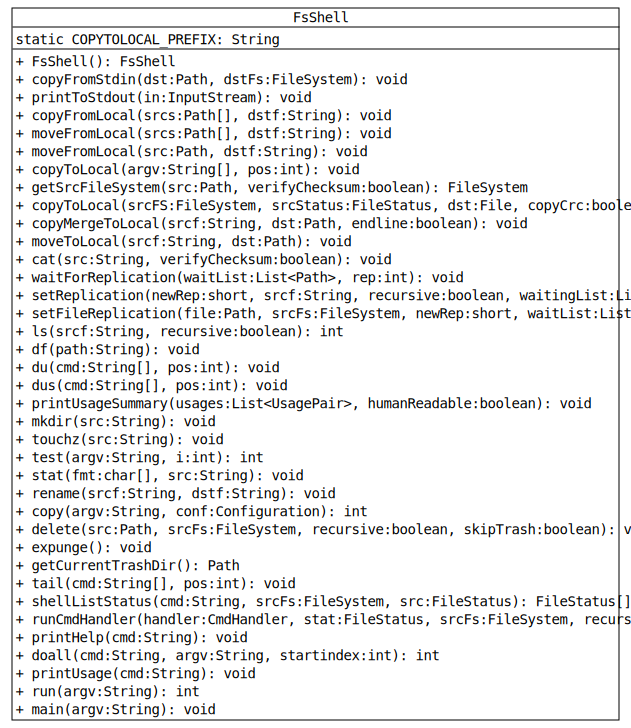
\includegraphics[width=\textwidth]{cdig/FsShell.png}
     
 向HFS中的文件系统提供命令行访问接口. 

    \begin{XeMethod}{\XePublic}{FsShell}{FsShell}
         
 以空的配置构造实例 

    \end{XeMethod}

    \begin{XeMethod}{\XePrivate}{void}{copyFromStdin}
         
 从stdin复制到指定\emph{FileSystem}的指定文件.

    \end{XeMethod}

    \begin{XeMethod}{\XePrivate}{void}{printToStdout}
         
 打印到stdout.

    \end{XeMethod}

    \begin{XeMethod}{}{void}{copyFromLocal}
         
 将本地文件添加到HFS.

    \end{XeMethod}

    \begin{XeMethod}{}{void}{moveFromLocal}
         
 从本地移动多个文件到目标文件系统.

    \end{XeMethod}

    \begin{XeMethod}{}{void}{moveFromLocal}
         
 从本地移动一个文件到目标文件系统.

    \end{XeMethod}

    \begin{XeMethod}{}{void}{copyToLocal}
         
 获取匹配模式的所有文件, 并将之复制到本地.
 源文件会被保存,当拷贝多个文件时,目标位置必须是一个文件夹,
 否则会抛出IOException异常。

    \end{XeMethod}

    \begin{XeMethod}{\XePrivate}{FileSystem}{getSrcFileSystem}
         
 返回src和conf对应的\emph{FileSystem},如果目标\emph{FileSystem.}支持校验和,则设置校验和。

    \end{XeMethod}

    \begin{XeMethod}{\XePrivate}{void}{copyToLocal}
         
 将\emph{FileSystem}中的文件拷贝到本地。

    \end{XeMethod}

    \begin{XeMethod}{}{void}{copyMergeToLocal}
         
 将符合srcf的模式的文件均拷贝到本地,合并为一个文件,源文件将被保留,
 此方法在合并时,可以指定是否在每个被合并的文件末尾加入一行来
 区分每个文件。

    \end{XeMethod}

    \begin{XeMethod}{}{void}{moveToLocal}
         
 获取并拷贝srcf指定的文件到本地目录,并且删除源文件。
 但此方法尚未被实现。

    \end{XeMethod}

    \begin{XeMethod}{}{void}{cat}
         
 获取所有的符合srcf模式的文件,并显示到\emph{stdout}

    \end{XeMethod}

    \begin{XeMethod}{}{void}{waitForReplication}
         
 等待所有的在waitlist中的文件,直到其副本数量达到rep

    \end{XeMethod}

    \begin{XeMethod}{}{void}{setReplication}
         
 改变一个文件的副本数。recursive选项用于递归改变目录下所有文件的副本数。

    \end{XeMethod}

    \begin{XeMethod}{\XePrivate}{void}{setFileReplication}
         
 为文件设置副本数量

    \end{XeMethod}

    \begin{XeMethod}{\XePrivate}{int}{ls}
         
 即unix系统上的ls命令,获取符合<i>srcf</i>模式的文件的状态

    \end{XeMethod}

    \begin{XeMethod}{}{void}{df}
         
 显示包含path的文件系统的分区大小

    \end{XeMethod}

    \begin{XeMethod}{}{void}{du}
         
 显示所有符合输入模式的文件的大小

    \end{XeMethod}

    \begin{XeMethod}{}{void}{dus}
         
 显示输入模式匹配的文件和文件目录的基本信息。

    \end{XeMethod}

    \begin{XeMethod}{\XePrivate}{void}{printUsageSummary}
         
 打印文件使用量的信息,此方法被\emph{du}命令使用。

    \end{XeMethod}

    \begin{XeMethod}{}{void}{mkdir}
         
 创建一个目录

    \end{XeMethod}

    \begin{XeMethod}{}{void}{touchz}
         
 在指定的src位置创建一个0长度的文件。
 此命令在未来版本将会仿照unix中的touch命令。

    \end{XeMethod}

    \begin{XeMethod}{}{int}{test}
         
 测试文件的类型

    \end{XeMethod}

    \begin{XeMethod}{}{void}{stat}
         
 将path的统计信息按照指定的格式输出
 格式字串:
 %b: 文件的block数量
 %n: 文件名
 %o: block大小
 %r: 副本数量
 %y: UTC 时间,格式为yyyy-MM-dd HH:mm:ss
 %Y: 毫秒数,从January 1, 1970 UTC开始

    \end{XeMethod}

    \begin{XeMethod}{}{void}{rename}
         
 移动/重命名文件,当一次移动多个文件时,目标位置必须是一个目录,否则会抛出
 \emph{IOException}

    \end{XeMethod}

    \begin{XeMethod}{\XePrivate}{int}{copy}
         
 复制文件,当一次复制多个文件时,目标位置必须是一个目录,否则会抛出

    \end{XeMethod}

    \begin{XeMethod}{\XePrivate}{void}{delete}
         
 删除src指定的文件,可以指定是否递归删除,可以指定是否移入垃圾箱

    \end{XeMethod}

    \begin{XeMethod}{\XePrivate}{void}{expunge}
         
 清空垃圾桶

    \end{XeMethod}

    \begin{XeMethod}{\XePublic}{Path}{getCurrentTrashDir}
         
 返回与这个FsShell对象相关的\emph{Trash}对象

    \end{XeMethod}

    \begin{XeMethod}{\XePrivate}{void}{tail}
         
 解析输入的命令,并执行tail命令

    \end{XeMethod}

    \begin{XeMethod}{\XePrivate}{FileStatus[]}{shellListStatus}
         
 返回src指定的文件夹所在的目录的所有文件的\emph{FileStatus}
 对象.

    \end{XeMethod}

    \begin{XeMethod}{\XePrivate}{int}{runCmdHandler}
         
 对一个CommandHandler执行其对应的命令,如果recursive选项为ture,则会递归执行

    \end{XeMethod}

    \begin{XeMethod}{\XePrivate}{void}{printHelp}
         
 根据不同的cmd来输出对应的帮助信息。

    \end{XeMethod}

    \begin{XeMethod}{\XePrivate}{int}{doall}
         
 对argv中从startindex开始的所有参数,执行cmd指定的命令。

    \end{XeMethod}

    \begin{XeMethod}{\XePrivate}{void}{printUsage}
         
 打印指定cmd的使用格式。

    \end{XeMethod}

    \begin{XeMethod}{\XePublic}{int}{run}
         
 Shell命令的主要处理函数,该函数会根据输入指令的不同,调用具体的处理函数。

    \end{XeMethod}

    \begin{XeMethod}{\XePublic}{void}{main}
         
 hadoop文件系统Shell接口的主要入口函数

    \end{XeMethod}


    \begin{XeInnerClass}{CmdHandler}
\includegraphics[width=\textwidth]{cdig/CmdHandler.png}
         
 该类会在给定的\emph{FileStatus}对象上运行,可以
 被用来执行chmod,chown等多种操作。
 例如在\emph{FsShellPermissions}类中,此类
 被继承为\emph{ChmodHandler</code>和<code>CmdHandler}

    \end{XeInnerClass}
    \begin{XeInnerClass}{DelayedExceptionThrowing}
\includegraphics[width=\textwidth]{cdig/DelayedExceptionThrowing.png}
         
 该类的作用是累积发生的Exception,等到指定的时间再进行抛出。
 例如在ls命令中,首先会逐条显示文件的信息,然后再抛出异常。

    \end{XeInnerClass}
    \begin{XeInnerClass}{UsagePair}
\includegraphics[width=\textwidth]{cdig/UsagePair.png}
         
 工具类,用作du的输出

    \end{XeInnerClass}
\end{XeClass}
